\documentclass[submit]{harvardml}

% You don't need to change these.
\course{CS181-S19}
\assignment{Assignment \#5}
\duedate{11:59pm April 19, 2019}
\newcommand{\attr}[1]{\textsf{#1}}
\usepackage[OT1]{fontenc}
\usepackage[colorlinks,citecolor=blue,urlcolor=blue]{hyperref}
\usepackage[pdftex]{graphicx}
\usepackage{subfig}
\usepackage{fullpage}
% \usepackage{palatino}
% \usepackage{mathpazo}
\usepackage{amsmath}
\usepackage{amssymb}
\usepackage{color}
\usepackage{todonotes}
\usepackage{listings}
\usepackage{common}
\usepackage{bm}
\usepackage{enumitem}
\usepackage{tikz}
\usepackage{xifthen}

\usepackage[mmddyyyy,hhmmss]{datetime}

\definecolor{verbgray}{gray}{0.9}

\lstnewenvironment{csv}{%
  \lstset{backgroundcolor=\color{verbgray},
  frame=single,
  framerule=0pt,
  basicstyle=\ttfamily,
  columns=fullflexible}}{}

\newcommand{\mueps}{\mu_{\epsilon}}
\newcommand{\sigeps}{\sigma_{\epsilon}}
\newcommand{\mugam}{\mu_{\gamma}}
\newcommand{\siggam}{\sigma_{\gamma}}
\newcommand{\muzp}{\mu_{p}}
\newcommand{\sigzp}{\sigma_{p}}
\newcommand{\gauss}[3]{\frac{1}{2\pi#3}e^{-\frac{(#1-#2)^2}{2#3}}}


\begin{document}
\begin{center}
{\Large Homework 5: Graphical Models, MDPs}\\
\end{center}

\subsection*{Introduction}

% FDV: Add useful readings here.

There is a mathematical component and a programming component to this
homework.  Please submit your \textbf{tex, PDF, and Python files} to
Canvas, and push all of your work to your GitHub repository. If a
question requires you to make any plots, please include those in the
writeup.

\newpage

\section*{Bayesian Networks [7 pts]}
\begin{problem}

  % FDV: Minor notation changes + changed the network.  Adjust the
  % solutions for the new network with the new names.

  \noindent In this problem we explore the conditional independence
  properties of a Bayesian Network.  Consider the following Bayesian
  network representing a student's work. Each random variable is
  binary (true/false).
 %
%\vspace{0.2in}
\begin{center}
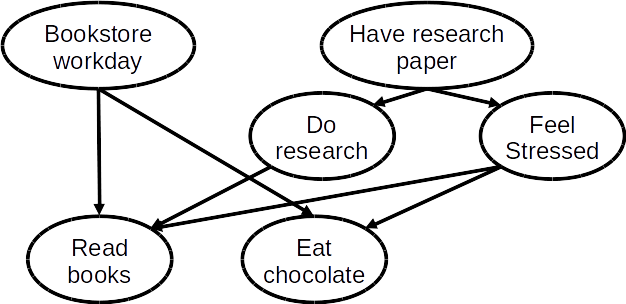
\includegraphics[width=3in]{bn.png}
\end{center}
%\vspace{0.2in}

The random variables are:
%
\begin{itemize}
\item \attr{Have research paper}: Does the student have a research paper?
\item \attr{Do Research}: Is the student doing research?
\item \attr{Feel Stressed}: Is the student feeling stressed?
\item \attr{Bookstore Workday}: Is the student working at the bookstore?
\item \attr{Read Books}: Is the student reading a book?
\item \attr{Eat Chocolate}: Is the student eating chocolate?
\end{itemize}

\medskip

For the following questions, $A \perp B$ means that events A and B are
independent and $A \perp B | C$ means that events A and B are independent
conditioned on C. Use the concept of d-separation to answer the
questions and show your work.

%
\begin{enumerate}
\item Is $\attr{Bookstore Workday} \perp \attr{Have research paper}$?
  If NO, give intuition for why.
%
%
\item Is $\attr{Bookstore Workday} \perp \attr{Have research
  paper}\given \attr{Read Books}$? If NO, give intuition for why.
%
%
\item Is $\attr{Do Research} \perp \attr{Eat Chocolate}$? If NO, give
  intuition for why.
%
\item Is $\attr{Do Research} \perp \attr{Eat Chocolate} \given
  \attr{Feel Stressed}$? If NO, give intuition for why.
%
\item Suppose the student has done some mindfulness exercises to avoid
  stress eating.  Now, when they are stressed, they read (fun) books
  but don't eat chocolate.  Draw the modified network.
%
%
\item For this modified network, is $\attr{Do Research} \perp
  \attr{Eat Chocolate}$? If NO, give an intuition why.  If YES,
  describe what observations (if any) would cause them to no longer be
  independent.
%
\end{enumerate}
\end{problem}
\subsection*{Solution}

For the following, I used the picture from UC Berkeley's CS 188 posted on Piazza to classify paths as active or inactive.

\begin{enumerate}
\item We have that $\boxed{\attr{Bookstore Workday} \perp \attr{Have research paper}}$ since there are no active paths between these nodes. \attr{Bookstore Workday} points into \attr{Read books} and \attr{Eat Chocolate}, but both of these nodes are unobserved descendents of \attr{Have research paper}. Hence, the path is inactive.

\item We have that $\boxed{\attr{Bookstore Workday} \not\perp \attr{Have research
  paper}\given \attr{Read Books}}$ since this creates an active path. To gain intuition, consider that \attr{Read books} is true and \attr{Bookstore Workday} is false. Then, we know \attr{Read books} must be true from \attr{Do research} or \attr{Feel Stressed}, which means \attr{Have research
  paper} will be true. Hence, conditional on \attr{Read books}, knowing something about \attr{Bookstore workday} tells us something about \attr{Have research paper} and vice versa.

\item We have that $\boxed{\attr{Do Research} \not\perp \attr{Eat Chocolate}}$ because there is an active path from \attr{Do Research} to \attr{Have research paper} to \attr{Feel stressed} to \attr{Eat Chocolate}. To gain intuition, consider that if \attr{Do research} is true, then we know \attr{Have research paper} is true, (or this becomes vary likely, depending on how we specify the network). Then, if \attr{Have research paper} is true, we know that \attr{Feel stressed} is also likely true. This in turn means that \attr{Eat chocolate} is likely to be true. Hence, knowing information about \attr{Do Research} gives us information about \attr{Eat chocolate}, so these two are not independent.

\item We have that $\boxed{\attr{Do Research} \perp \attr{Eat Chocolate} \given
  \attr{Feel Stressed}}$ since conditioning on \attr{Feel Stressed} kills the active path. To gain intuition\footnote{oops, wasn't supposed to give intuition here...}, consider that the only inputs to  \attr{Eat chocolate} are \attr{Bookstore workday} and  \attr{Feel stressed}.  \attr{Do Research} is independent of  \attr{Bookstore workday}, so it cannot influence  \attr{Eat chocolate} via this node. However, \attr{Do Research} does have a common ancestor of \attr{Eat chocolate} which is \attr{Have research paper}. Hence, if \attr{Do Research} is true, we expect \attr{Have research paper} to be more likely to be true meaning \attr{Feel stressed} is more likely to be true and similarly with \attr{Eat chocolate}. Hence,  \attr{Do Research} tells us information about \attr{Eat chocolate}. However, conditional on \attr{Feel stressed}, learning about \attr{Do Research} tells us nothing because we do not care if \attr{Feel stressed} is more likely to be true or not: we know exactly what it is! Hence, conditional on \attr{Feel stressed}, \attr{Do research} and \attr{Eat chocolate} are independent.

\item The modified network is depicted below. It is exactly the same, but now no edge exists between   \attr{Feel stressed} and \attr{Eat chocolate}.

\begin{center}
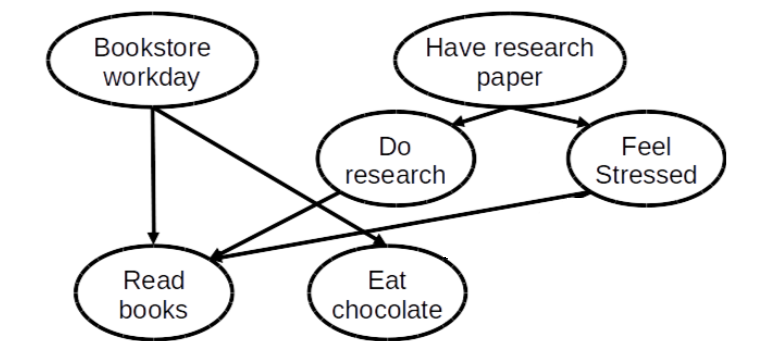
\includegraphics[scale=0.8]{1_5.png}
\end{center}

\item  In this modified network, we have that $\boxed{\attr{Do Research} \perp
  \attr{Eat Chocolate}}$. However, if we observe $\boxed{\attr{Read books} }$ these two nodes will become dependent since this would create an active path from \attr{Do Research} to \attr{Read books} to  \attr{Bookstore workday} to \attr{Eat chocolate}. Specifically, if we observe that \attr{Read books} is false and know that \attr{Do research} is true, than it is likely that \attr{Bookstore workday} is false meaning it is also likely that \attr{Eat chocolate} is false. Hence, conditional on \attr{Read books}, learning the value of \attr{Do research} gives us information about \attr{Eat chocolate}.
  
\end{enumerate}

\newpage

\section*{Kalman Filters [7 pts]}

% FDV: This problem is the same as last year.  Take a close look for
% anything that could have been confusing.

\begin{problem}
In this problem, you will implement a one-dimensional Kalman filter.
Assume the following dynamical system model:
  \begin{eqnarray*}
    z_{t+1} &= z_{t} + \epsilon_{t} \\
    x_{t} & = z_{t} + \gamma_{t}
  \end{eqnarray*}
  where $z$ are the hidden variables and $x$ are the observed
  measurements.  The random variables $\epsilon$ and $\gamma$ are
  drawn from the following Normal distributions:
  \begin{eqnarray*}
    \epsilon_t &\sim& N(\mueps,\sigeps) \\
    \gamma_t &\sim& N(\mugam,\siggam)
  \end{eqnarray*}
  where $\mueps = 0$, $\sigeps=0.05$, $\mugam = 0$ and $\siggam=1.0$

You are provided with the observed data $x$ and the hidden data $z$ in
\texttt{kf-data.csv}, and the prior on the first hidden state is $p(z_0)$ =
N($\muzp$,$\sigzp$) where $\muzp = 5$ and $\sigzp=1$

    \begin{enumerate}
      \item The distribution $p(z_t|x_0...x_t)$ will be Gaussian
        $N(\mu_t,\sigma^2_t)$. Derive an iterative update for the mean
        $\mu_t$ and variance $\sigma^2_t$ given the mean and variance
        at the previous time step ($\mu_{t-1}$ and $\sigma^2_{t-1}$).

       \item Implement this update and apply it to the observed data
         above (do not use the hidden data to find these
         updates). Provide a plot of $\mu_t$ over time as well as a
         $2\sigma_t$ interval around $\mu_t$ (that is $\mu_t \pm
         2\sigma_t$).  Does the Kalman filter ``catch up'' to the true
         hidden object?

       \item Repeat the same process but change the observation at
         time $t=10$ to $x_{t=10}=10.2$ (an extreme outlier
         measurement).  How does the Kalman filter respond to this
         outlier?

       \item Comment on the misspecification of dynamical system model
         for these data.  Based on the previous two parts, how does
         this misspecification affect the predictions?

\end{enumerate}
\end{problem}
\subsection*{Solution}

\begin{enumerate}

\item We wish to find the mean and variance of $p(z_t|x_0\dots x_t)$ given $u_{t-1}$ and $\sigma^2_{t-1}$. By Bayes' rule, we have 

$$p(z_t|x_0\dots x_t) = \frac{p(x_t|x_0\dots x_{t-1}, z_t)p(z_t|x_0\dots x_{t-1})}{p(x_t|x_0\dots x_{t-1})} \propto p(x_t|x_0\dots x_{t-1}, z_t)p(z_t|x_0\dots x_{t-1}) $$

where I will ignore the denominator since it is a function of only the observed data. Now, using the fact that in our model $x_t$ only depends on $z_t$, we can drop some of the above conditioning. We have that

$$p(z_t|x_0\dots x_t) \propto \underbrace{p(x_t|z_t)}_{N(x_t; z_t+\mu_\gamma, \sigma^2_\gamma)} p(z_t|x_0\dots x_{t-1}) $$

Using LOTP and conditioning on all possible values of $z_{t-1}$, we can expand the second term as

$$p(z_t|x_0\dots x_{t-1}) = \int_{-\infty}^\infty p(z_t|x_0\dots x_{t-1},z_{t-1})p(z_{t-1}| x_0\dots x_{t-1}) dz_{t-1}  $$

Since $z_t$ only depends on $z_{t-1}$, this becomes

$$ = \int_{-\infty}^\infty \underbrace{p(z_t|z_{t-1})}_{N(z_t; z_{t-1}+\mu_\epsilon, \sigma^2_\epsilon)} \underbrace{p(z_{t-1}| x_0\dots x_{t-1})}_{N(z_{t-1}; \mu_{t-1}, \sigma^2_{t-1})} dz_{t-1}  $$

Now, note that $N(z_t; z_{t-1}+\mu_\epsilon, \sigma^2_\epsilon) = N(-z_t; -z_{t-1}-\mu_\epsilon, \sigma^2_\epsilon) = N(z_{t-1}; z_t-\mu_\epsilon, \sigma^2_\epsilon)$. Hence, we have

$$p(z_t|x_0\dots x_{t-1}) =\int_{-\infty}^\infty \underbrace{p(z_t|z_{t-1})}_{N(z_{t-1}; z_t-\mu_\epsilon, \sigma^2_\epsilon)} \underbrace{p(z_{t-1}| x_0\dots x_{t-1})}_{N(z_{t-1}; \mu_{t-1}, \sigma^2_{t-1})} dz_{t-1}  $$

At this point, it will help to evaluate the product of two general Gaussian PDF's evaluated at $x$. Specifically, for $N(x;a,\sigma^2_a)$ and $N(x;b,\sigma^2_b)$ Gaussians, the product of their PDFs is

$$\frac{1}{\sqrt{2\pi\sigma^2_a}}\exp\big(-\frac{(x-a)^2}{2\sigma^2_a}\big)\frac{1}{\sqrt{2\pi\sigma^2_b}}\exp\big(-\frac{(x-b)^2}{2\sigma^2_b}\big) $$

Now, focusing on the (negated) inside of the exponential terms and completing the square, we will get 

$$\frac{(x-a)^2}{2\sigma^2_a} + \frac{(x-b)^2}{2\sigma^2_b} = \frac{\sigma^2_a + \sigma^2_b}{2\sigma^2_a \sigma^2_b}x^2 - \frac{a\sigma^2_b+b\sigma^2_a}{\sigma^2_a\sigma^2_b}x +\frac{a^2\sigma^2_b + b^2\sigma^2_a}{2\sigma^2_a\sigma^2_b}$$ 

$$ = \underbrace{\frac{\sigma^2_a+\sigma^2_b}{2\sigma^2_a\sigma^2_b}\big(x-\frac{a\sigma^2_b +b\sigma^2_a}{\sigma^2_a+\sigma^2_b} \big)^2}_{\propto\textrm{Gaussian over x}} + \underbrace{\frac{(a-b)^2}{2(\sigma^2_a+\sigma^2_b)}}_{\propto\textrm{Gaussian over a}}$$

From the above, as indicated, we have two terms that are proportional to a Gaussian over $x$ and a Gaussian over $a$, or equivalently $b$. In fact, we can actually conclude that these are both valid PDFs since they will need to normalize.\footnote{I'm not actually positive why this works out, but my results match those found in the Tina-Vision resource suggested by TF's and results in Bishop...so the normalization constants must work out!} The Gaussian over $x$ has mean and variance

$$ \mu = \frac{a\sigma^2_b + b\sigma^2_a}{\sigma^2_a + \sigma^2_b}, \sigma^2 = \frac{\sigma^2_a\sigma^2_b}{\sigma^2_a+\sigma^2_a}$$

while the Gaussian over $a$ has mean and variance

$$\mu = b, \sigma^2 = \sigma^2_a + \sigma^2_b $$

Now, using this result to evaluate the integral in question above, we realize that the integrand can be rewritten as a Gaussian over $z_{t-1}$ and a Gaussian over $\mu_{t-1}$. Since we are integrating over all values of $z_{t-1}$, the first Gaussian will integrate to $1$. The second Gaussian is a constant with respect to the integral, so it can be pulled out. Specifically, we will have

$$p(z_t|x_0\dots x_{t-1}) = N(\mu_{t-1}; z_{t} - \mu_\epsilon, \sigma^2_\epsilon + \sigma^2_{t-1}) = N(-\mu_{t-1}; -z_{t} + \mu_\epsilon, \sigma^2_\epsilon + \sigma^2_{t-1}) = N(z_t; \mu_{t-1} + \mu_\epsilon, \sigma^2_\epsilon + \sigma^2_{t-1})  $$

Also, note that $p(x_t|z_t) = N(x_t;z_t+\mu_\gamma,\sigma^2_\gamma) = N(-x_t; -z_t-\mu_\gamma,\sigma^2_\gamma) = N(z_t; x_t-\mu_\gamma,\sigma^2_\gamma)$. Now, we realize that

$$p(z_t|x_0\dots x_t) \propto \underbrace{p(x_t|z_t)}_{N(z_t; x_t-\mu_\gamma,\sigma^2_\gamma)} \underbrace{p(z_t|x_0\dots x_{t-1})}_{N(z_t; \mu_{t-1} + \mu_\epsilon, \sigma^2_\epsilon + \sigma^2_{t-1}) } $$

Again, using the general formula for the product of two Gaussians evaluated at the same value, we realize that this is equivalent to a Gaussian over $z_t$ multiplied by a Gaussian over $\mu_{t-1} + \mu_{\epsilon}$. Note that we are just working with proportionality here, so the second Gaussian can be ignored since it is constant wrt $z_t$ and we are only concerned with the distribution of $z_t$. Hence, from my equations above, we conclude that $p(z_t|x_0\dots x_t)$ is a Gaussian over $z_t$ with the following mean and variance

$$ \boxed{\mu_t = \frac{(x_t-\mu_\gamma)(\sigma^2_\epsilon + \sigma^2_{t-1}) + (\mu_{t-1} + \mu_\epsilon)\sigma^2_\gamma}{\sigma^2_\gamma + \sigma^2_\epsilon + \sigma^2_{t-1}}, \sigma^2_t = \frac{\sigma^2_\gamma(\sigma^2_\epsilon + \sigma^2_{t-1})}{\sigma^2_\gamma+\sigma^2_\epsilon + \sigma^2_{t-1}}}$$

Plugging in the values we were given in this problem, these becomes

$$ \boxed{\mu_t = \frac{x_t(0.0025 + \sigma^2_{t-1}) + \mu_{t-1}}{1.0025 + \sigma^2_{t-1}}, \sigma^2_t = \frac{0.0025 + \sigma^2_{t-1}}{1.0025 + \sigma^2_{t-1}}}$$

So, we have found the desired iterative update. Now, we need to solve for our starting conditions. By Bayes' rule, we know

$$p(z_0|x_0) =\frac{p(x_0|z_0)p(z_0)}{p(x_0)} \propto p(x_0|z_0)p(z_0)$$

Again, we ignore the denominator since it is a function of the observed data. We are given that $p(z_0) = N(\mu_p,\sigma^2_p)$. Additionally, we know that $p(x_0|z_0) = N(x_0; z_0  + \mu_\gamma, \sigma^2_\gamma) =  N(-x_0; -z_0  - \mu_\gamma, \sigma^2_\gamma) = N(z_0; x_0  - \mu_\gamma, \sigma^2_\gamma) $. Hence, we have that 

$$p(z_0|x_0)  \propto \underbrace{p(x_0|z_0)}_{N(z_0; x_0  - \mu_\gamma, \sigma^2_\gamma)} \underbrace{p(z_0)}_{N(z_0;\mu_p,\sigma^2_p)}$$

and from the formula I derived above, we conclude that this is equivalent to the product of a Gaussian over $z_0$ and a Gaussian over $\mu_p$. We can ignore the second Gaussian since it is a constant wrt $z_0$ and we are working with a proportionality. Furthermore, since the r.h.s. is a valid PDF over $z_0$, we conclude the l.h.s. must be as well and the proportionality constant will work out (this is the same logic we used above). So, we have $p(z_0)$ is a Gaussian with mean and variance

$$\boxed{\mu_0 = \frac{(x_0-\mu_\gamma)\sigma^2_p + \mu_p\sigma^2_\gamma}{\sigma^2_\gamma + \sigma^2_p }, \sigma^2_0 =  \frac{\sigma^2_\gamma\sigma^2_p}{\sigma^2_\gamma + \sigma^2_p}}$$

Plugging in the actual values for this problem, these become 

$$\boxed{\mu_0 = \frac{x_0 + 5}{2}, \sigma^2_0 =  \frac{1}{2}}$$

\item Below is a graph of my implementation of the Kalman Filter on the observed data. The blue points are the hidden data and the orange line is the mean of $p(z_t|x_0\dots x_t)$, $\mu_t$, with $\pm 2\sigma_t$ errorbars. 

\begin{center}
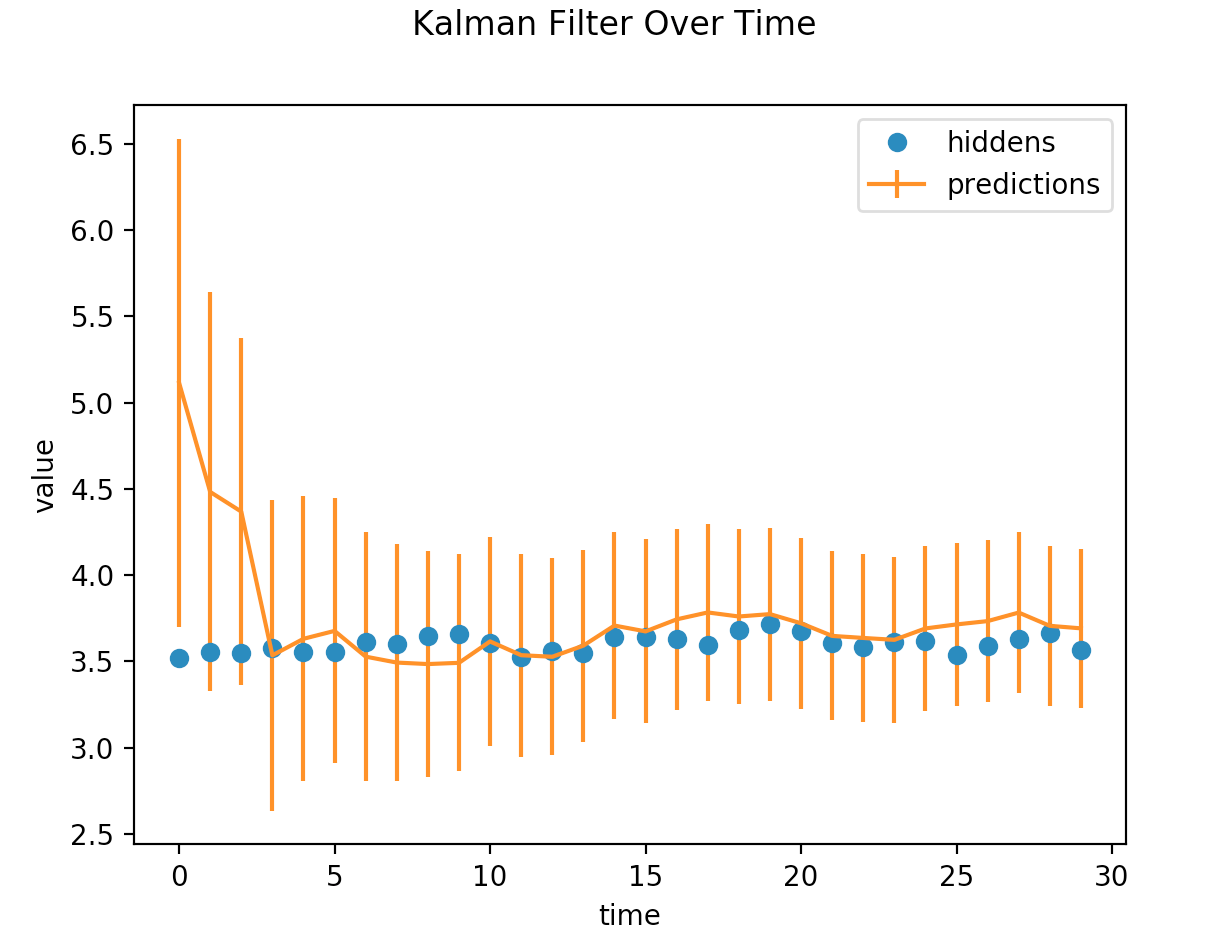
\includegraphics[scale=0.7]{2_2.png}
\end{center}

As can be seen, the Kalman filter does indeed ``catch up" to the true hiddens. By the fourth observation the Kalman Filter mean is practically equal to the hidden, and it stays very close to the hidden values as time progresses.

\item Below is the same graph but now $x_{t=10} = 10.2$, far outside of two standard deviations of the Kalman Filter mean. 

\begin{center}
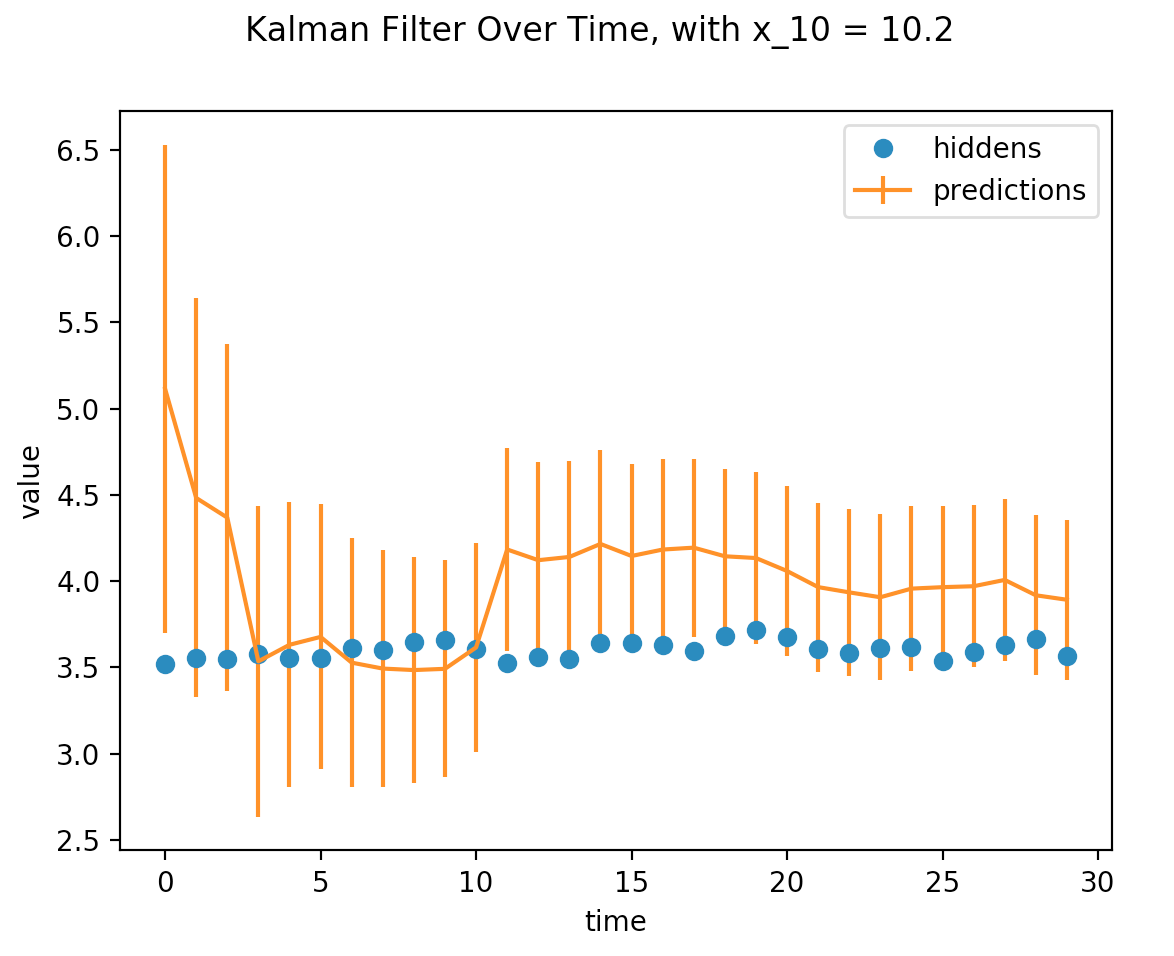
\includegraphics[scale=0.7]{2_3.png}
\end{center}

As can be seen, the Kalman filter responds poorly to this outlier and consistently overestimates the hiddens afterwards, even after nearly 20 additional observations. The Kalman filter mean does move closer to the hiddens by $t=29$, but not by very much.

\item There are several ways this model can be misspecified. Specifically, our parameters are $\mu_p, \sigma_p, \mu_\epsilon, \sigma_\epsilon, \mu_\gamma$, and $\sigma_\gamma$. From looking at the above graphs, its clear that we have misspecified $\mu_p$ or $\sigma_p$ since $z_0$ is well beyond two standard deviations below the mean, and we are using a Gaussian model. This means if our model is correct, we'd expect this to happen less than 5\% of the time, roughly. So, it's likely we misspecified $\mu_p$ or $\sigma_p$ or perhaps both. However, the mean of the Kalman Filter is able to catch up to the hiddens quickly. So with regard to the prior, it seems our model is not very sensitive to misspecification.

In 2.3, we consider the scenario where we observe $x_{t=10}= 10.2$, which is far from what we would expect it to be since our model assumes $x_t \sim N(z_t + \mu_\gamma, \sigma^2_\gamma) = N(z_t, 1)$. In this scenario we have left $z_t$ unchanged, and it is around 3.5. Hence, we realize that we have clearly misspecified $\mu_\gamma$, $\sigma_\gamma$, or both of these parameters because the probability of $x_{t=10}= 10.2$ when $x_{t=10} \sim N(3.53,1)$ is extremely small. Under this misspecification, our model does poorly to catch up to the true hiddens. Over the remaining 19 data point, the mean of $p(z_t|x_0 \dots x_t)$ remains relatively far away from the hidden values. 

Note that this scenario of $x_{t=10}= 10.2$ could also have occurred if $z_{10}$ had been a large value, which would have implied that $\mu_\epsilon$ or $\sigma_\epsilon$ or both were misspecified since $z_{10} \sim N(z_9 + \mu_\epsilon, \sigma^2_\epsilon) = N(3.61, 1)$. Thus, we can also conclude that misspecification of $\mu_\epsilon$ or $\sigma_\epsilon$ or both would lead to the mean of our Kalman Filter moving far away from the hidden values and failing to catch up for some time. All of this is to say that our model is sensitive to a misspecification of $\mu_\epsilon, \sigma_\epsilon, \mu_\gamma,$ or $\sigma_\gamma$, or a combination of misspecifying these parameters. Our predictions become poor under such misspecification.

To explore this more, I considered a few extra scenarios. Note that these scenarios do not cover all possible misspecifications, but they do offer some insight. 

\begin{center}
\begin{tabular}{ c c c }
 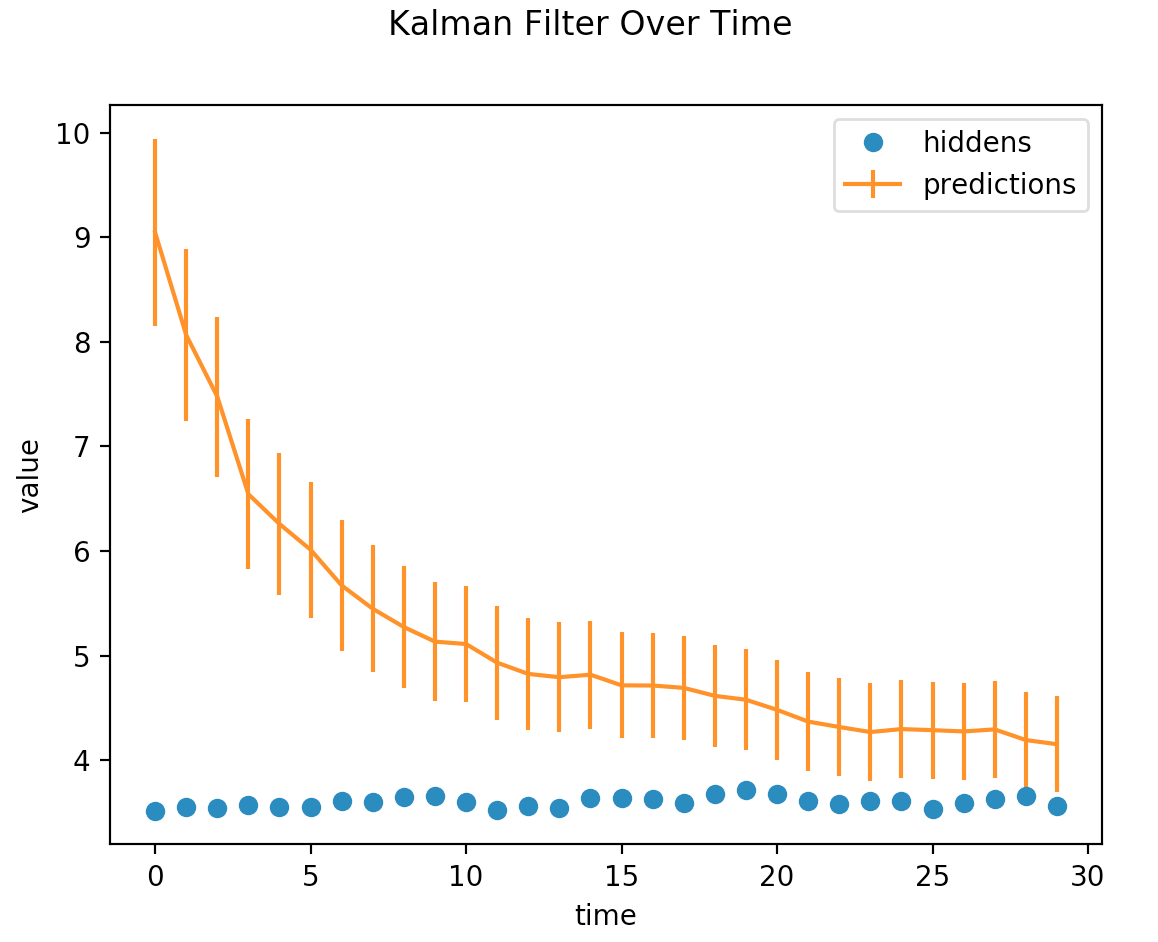
\includegraphics[scale=0.25]{a.png} & 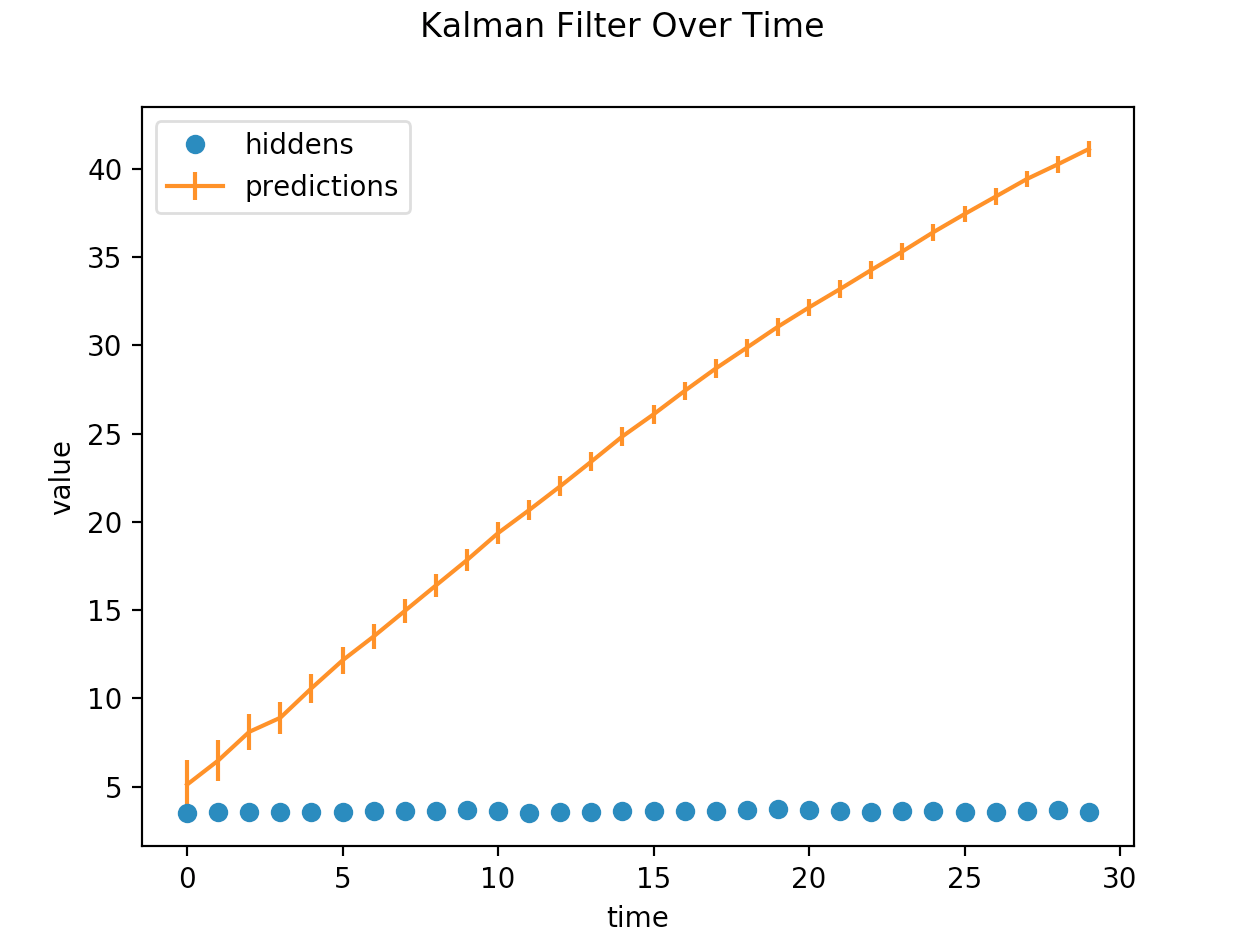
\includegraphics[scale=0.25]{b.png} & 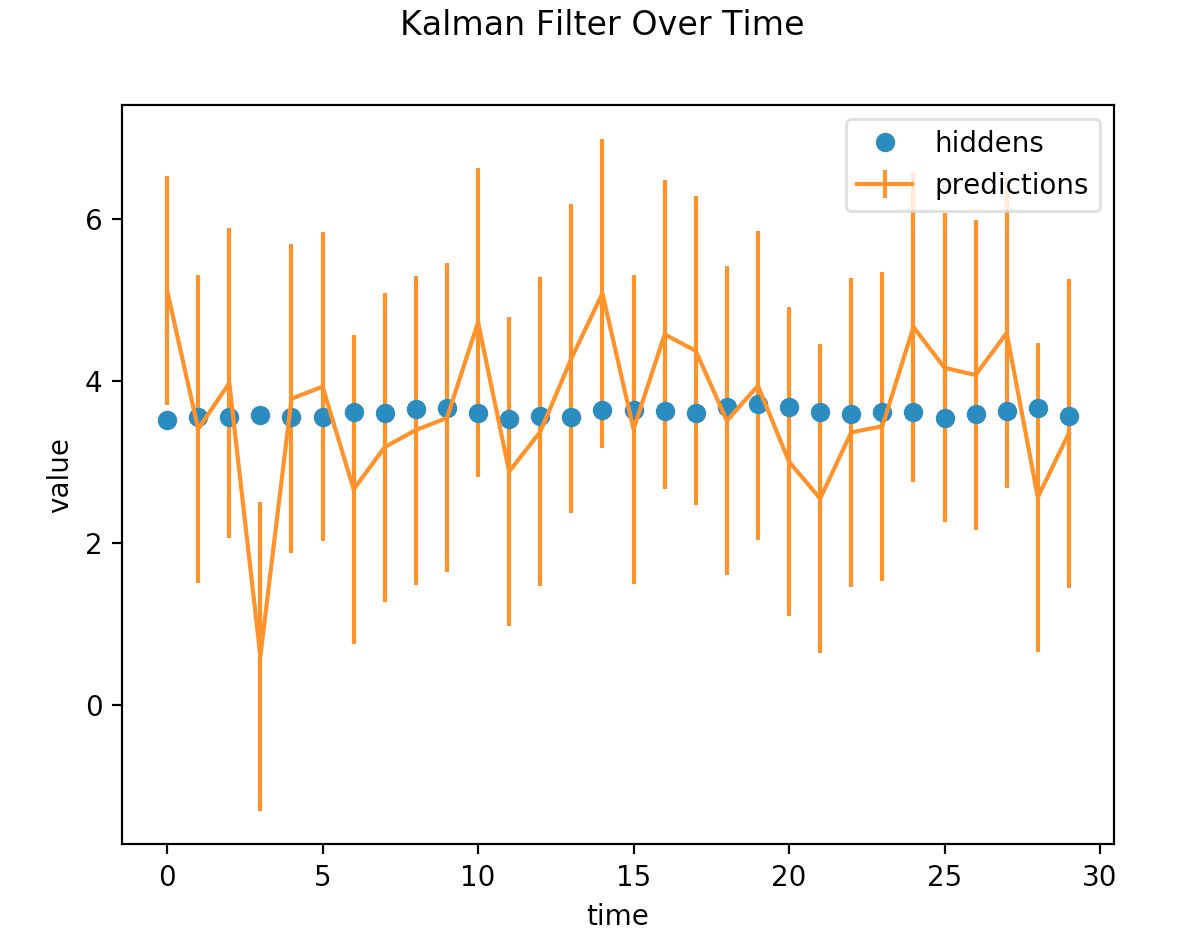
\includegraphics[scale=0.25]{c.png}  \\ 
 a) $\mu_p = 10, \sigma_p = 0.5$ & b) $\mu_\epsilon = 3$ & c) $\sigma_\epsilon = 3$ 
\end{tabular}
\end{center}

\begin{center}
\begin{tabular}{ c c }
 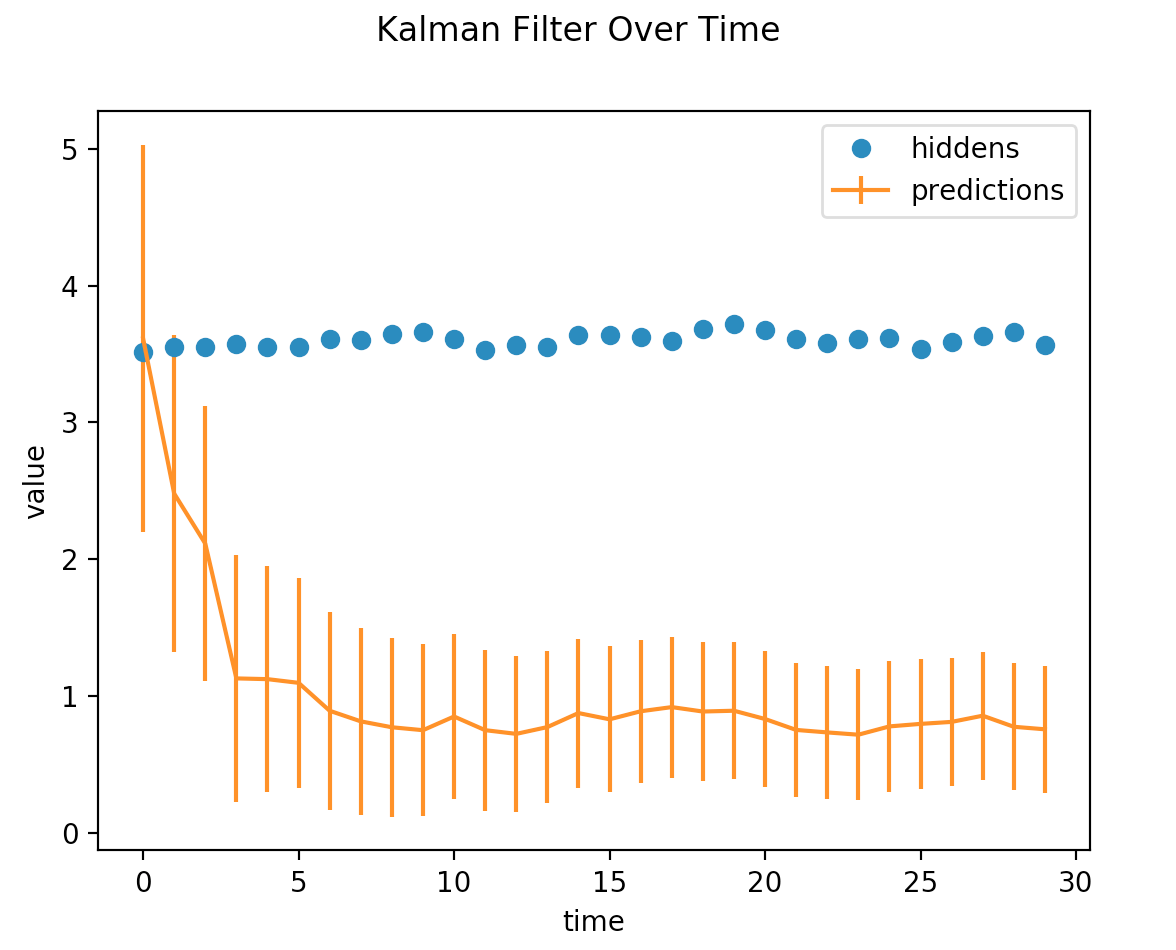
\includegraphics[scale=0.25]{d.png} & 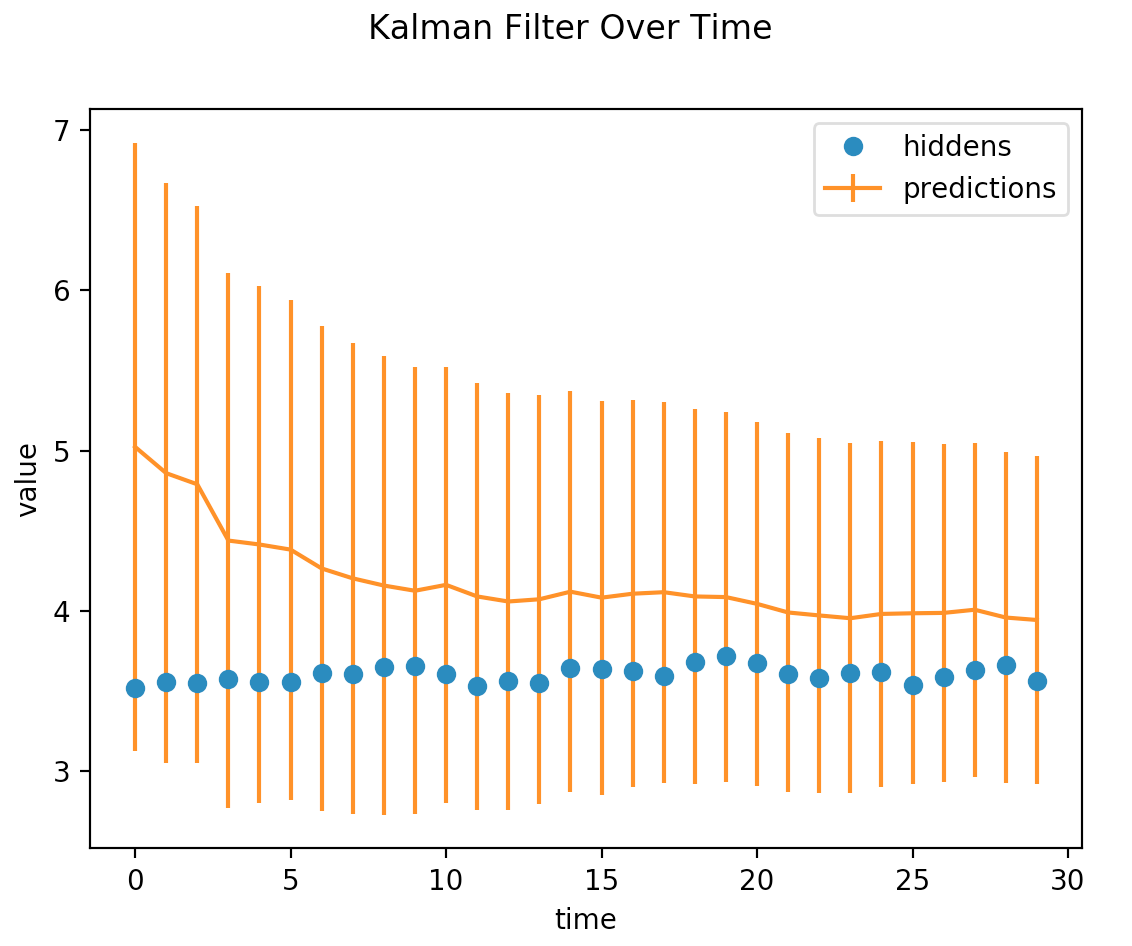
\includegraphics[scale=0.25]{e.png} \\ 
 d) $\mu_\gamma = 3$ & e) $\sigma_\gamma = 3$
\end{tabular}
\end{center}

I listed the only altered parameters below each graph. All other parameters are the same as they are in the problem statement. As can be seen, the Kalman Filter mean does quite well to catch up to the data even under the extreme misspecification of the prior in (a). It is not fully able to catch up to the hiddens by $t =29$, but it comes close. With all the other misspecifications, the Kalman Filter mean does a poor job getting close to the hiddens. It is especially bad under misspecifications of $\mu_\epsilon$ and $\mu_\gamma$. Misspecifications of $\sigma_\epsilon$ and $\sigma_\gamma$ seem to affect the rate at which the Kalman Filter can catch up to the data, and it's ability to stay close to the hiddens once it has made a fairly accurate prediction. 

\end{enumerate}

\newpage

\begin{problem}[Explaining Away, 7 pts]

  In this problem, you will carefully work out a basic example with
  the explaining away effect.  There are many derivations of this
  problem available in textbooks.  We emphasize that while you may
  refer to textbooks and other online resources for understanding how
  to do the computation, you should do the computation below from
  scratch, by hand.

  We have three binary variables, rain $r$, grass-wet $g$, and
  sprinkler $s$.  The conditional probability tables look like the
  following:
  \begin{eqnarray*}
    p(r = 1) &= 0.25 \\
    p(s = 1) &= 0.5 \\
    p(g = 1 | r = 0 , s = 0 ) &= 0 \\
    p(g = 1 | r = 1 , s = 0 ) &= .75 \\
    p(g = 1 | r = 0 , s = 1 ) &= .75 \\
    p(g = 1 | r = 1 , s = 1 ) &= 1
  \end{eqnarray*}

  \begin{enumerate}
    \item You check on the sprinkler without checking on the rain or
      the grass.  What is the probability that it is on?
    \item You notice it is raining and check on the sprinkler without
      checking the grass.  What is the probability that it is on?
    \item You notice that the grass is wet and go to check on the
      sprinkler (without checking if it is raining).  What is the
      probability that it is on?
    \item You notice that it is raining and the grass is wet.  You go
      check on the sprinkler.  What is the probability that it is on?
    \item What is the explaining away effect above?
    \end{enumerate}

\end{problem}

\subsection*{Solution}

  \begin{enumerate}
    \item The probability that the sprinkler is on in this scenario is simply its marginal probability. This is $\boxed{0.5}$.
        \item We wish to find $P(s=1|r=1)$. Note that the rain and the sprinkler are independent. So, by the definition of conditional probability, we have
        $$P(s=1|r=1) = \frac{P(s=1,r=1) }{P(r=1)} =  \frac{P(s=1)P(r=1) }{P(r=1)} = P(s=1) = 0.5 $$
        
        Thus, due to the independence between the sprinkler and the rain, this probability is also $\boxed{0.5}$.
        
    \item We wish to find $P(s=1|g=1)$. Using Bayes' rule, this is
    
    $$P(s=1|g=1) = \frac{P(g=1|s=1)P(s=1) }{p(g=1)} $$ 
    
    By LOTP, the numerator and denominator will be
    
    $$\textrm{numerator: } \big(P(g=1|s=1,r=0)P(r=0|s=1)+ P(g=1|s=1,r=1)P(r=1|s=1) \big)P(s=1) $$
    $$\textrm{denominator: } \big(P(g=1|s=1,r=0)P(r=0|s=1)+ P(g=1|s=1,r=1)P(r=1|s=1) \big)P(s=1) $$
    $$+ \big(P(g=1|s=0,r=0)P(r=0|s=0)+ P(g=1|s=0,r=1)P(r=1|s=0) \big)P(s=0) $$
    
    Then, since $P(s=1) = P(s=0)$, and since $s \perp r$, these become
    
    $$\textrm{numerator: } P(g=1|s=1,r=0)P(r=0)+ P(g=1|s=1,r=1)P(r=1) $$
    $$\textrm{denominator: } P(g=1|s=1,r=0)P(r=0)+ P(g=1|s=1,r=1)P(r=1) $$
    $$+ P(g=1|s=0,r=0)P(r=0)+ P(g=1|s=0,r=1)P(r=1)$$
    
    Plugging in the actual values for these, we have
    
    $$P(s=1|g=1) = \frac{0.75^2 + 1\times 0.25}{0.75^2 + 1\times 0.25 + 0 \times 0.75 + 0.75 \times 0.25} $$
    $$ = \frac{13}{16} = 0.8125$$
    
    Hence, we see that the desired probability is $\boxed{0.8125}$.
    
    \item We wish to find $P(s=1| g=1, r=1)$. Using conditional Bayes' rule, this is
    
    $$P(s=1| g=1, r=1) = \frac{P(g=1|s=1, r=1)p(s=1|r=1)}{p(g=1|r=1)} $$
    $$= \frac{1 \times 0.5}{p(g=1|r=1,s=0)p(s=0|r=1) + p(g=1|r=1,s=1)p(s=1|r=1) } $$
    
    Since $s \perp r$, this becomes 
    
    $$P(s=1| g=1, r=1) = \frac{1 \times 0.5}{p(g=1|r=1,s=0)p(s=0) + p(g=1|r=1,s=1)p(s=1) } =\frac{1 \times 0.5}{0.75 \times 0.5 + 1 \times 0.5 } $$
    
    $$= \frac{4}{7} \approx 0.571 $$  
    
    Hence, desired probability is about $\boxed{ 0.571}$ or $\frac{4}{7}$.
    
    \item The explaining away effect above is that conditioning on it raining in addition to the grass being wet in part 4 lowers the probability of the sprinkler being on (to 0.571) compared to when we found the probability of the sprinkler being on only conditioning on the grass being wet (which was 0.8125), found in part 3. This is because when we observe that the grass is wet, we know that this means that either the sprinkler is on, it is raining, or both. So, conditional on the grass being wet, the probability of the sprinkler being on and the probability of it raining are both high. However, when we observe that the grass is wet and that it is raining, the probability of the sprinkler being on goes down. This is because we have observed a reason for why the grass could be wet, and this observation ``explains away" the probability of the sprinkler being on. It is still possible that the sprinkler is on in this scenario, but we expect it to be on with much less probability because we have already observed a reason for why the grass is wet.
    
    \end{enumerate}


\newpage

\begin{itemize}
    \item Name: Zachary Dietz
    \item Email: zdietz@college.harvard.edu
    \item Collaborators: Theo Walker
    \item Approximately how long did this homework take you to complete (in hours): 10
\end{itemize}

\end{document}
